\PassOptionsToPackage{x11names,rgb,usenames,dvipsnames}{xcolor}
\documentclass[border=10pt]{standalone}
\usepackage{tikz}
\usepackage{amsmath}
\usetikzlibrary{calc,positioning,patterns,fit,intersections,decorations.pathreplacing}

\usepackage{tikz-dimline}
\usepackage{wasysym}

%-------------------------------------------------------------------------------------------------------------------------------------------------------------------------------- Shaded Pattern
% Adapted from the 'patterns' library: enlarged the distance between the lines from 4pt to 10pt
\pgfdeclarepatternformonly{north east lines wide}{\pgfqpoint{-1pt}{-1pt}}{\pgfqpoint{10pt}{10pt}}{\pgfqpoint{9pt}{9pt}}%
{
  \pgfsetlinewidth{0.4pt}
  \pgfpathmoveto{\pgfqpoint{0pt}{0pt}}
  \pgfpathlineto{\pgfqpoint{9.1pt}{9.1pt}}
  \pgfusepath{stroke}
}

%----------------------------------------------------------------------------------------------------------------------------------- Tikz Styles
\makeatletter
\tikzset{%
%--------------- Basic Styles
    rect/.style={inner sep=0pt,outer sep=0pt,align=center,shape=rectangle,draw,thick},
    shaded/.style={pattern=north east lines wide},
    OPSL/.style={dashed,Purple,ultra thick},
    symmetry/.style={dashed,thin},
%--------------- Laser Styles 
    mountingplate/.style={rect,fill=black!05!white,fit={(0,0)(6,9)},label=below:{\bfseries Mounting Plate}},
    toptica/.style={rect,draw=NavyBlue,fit={(0,0)(2,6)}, line width = 1pt,
				label={[align=center]above:{\color{NavyBlue}\bfseries Toptica\\ \color{NavyBlue}\bfseries GSL}}
			},
    ANULaser/.style={rect,dashed,Purple,ultra thick, fit={(0,0)(2.5,1)}, label=center:{\color{Purple}\bfseries ANU GSL}},
    breadboard/.style={rect,shaded,label=below:{\color{Orange!20!Red}\bfseries Breadboard},draw=Orange!20!Red,pattern color=Orange!20!Red},
    EOSbreadboard/.style={rect,shaded, minimum width = 9cm, minimum height = 1cm,
					label=above:{\color{PineGreen}\bfseries EOS Breadboard},
					draw=PineGreen,pattern color=PineGreen}
}
\makeatother


%----------------------------------------------------------------------------------------------------------------------------------- Document Start
\begin{document}

%----------------------------------------------------------------------------------------------------------------------------------- Picture Start
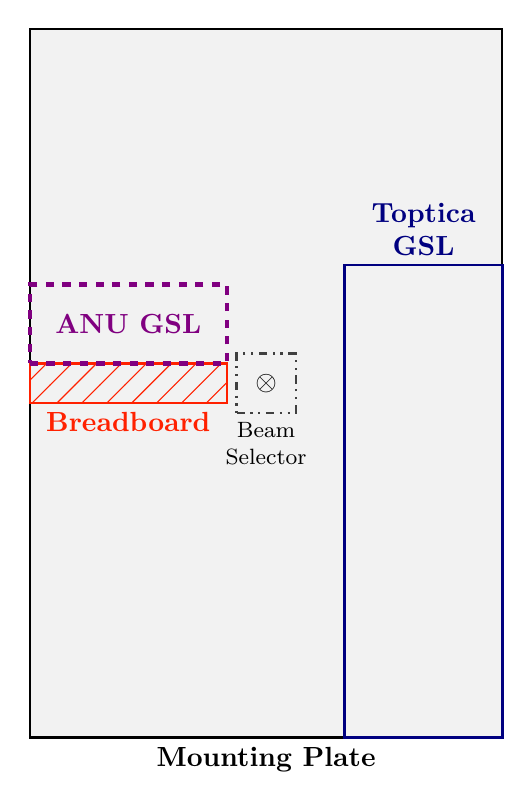
\begin{tikzpicture}[scale=1]

% Coordinates
\coordinate[label=below left:] (O) at (0,0);
\node[mountingplate] (MP) at (O) {};
\node[] at (O) {$\otimes$};
\node[rect, dash dot dot, minimum size = 0.75cm, darkgray, label={[align=center]below:{\footnotesize Beam\\[-0.5ex] \footnotesize  Selector}}] at (O) {};
\node[toptica, above left] at (MP.south east) {};
\node[breadboard,fit={(0,0)(2.5,0.5)},right] (nBB) at (MP.west) {};
\node[ANULaser, above] at (nBB.north) {};


%----------------------------------------------------------------------------------------------------------------------------------- Document/Picture End
\end{tikzpicture}
\end{document}